\documentclass[11pt, a4paper]{article}

% ── Packages ──────────────────────────────────────────────
\usepackage[margin=2.4cm]{geometry}
\usepackage[utf8]{inputenc}
\usepackage[T1]{fontenc}
\usepackage{lmodern}
\usepackage{booktabs}
\usepackage{tabularx}
\usepackage{array}
\usepackage{longtable}
\usepackage{enumitem}
\usepackage{tikz}
\usepackage{xcolor}
\usepackage{hyperref}
\usepackage{fancyhdr}
\usepackage{titlesec}
\usepackage{caption}
\usepackage{float}

% ── Colors ────────────────────────────────────────────────
\definecolor{primary}{HTML}{1A3A5C}
\definecolor{accent}{HTML}{2D7DD2}
\definecolor{lightgray}{HTML}{F4F4F4}
\definecolor{midgray}{HTML}{CCCCCC}
\definecolor{darktext}{HTML}{222222}
\definecolor{nodeblue}{HTML}{D6EAF8}
\definecolor{nodegreen}{HTML}{D5F5E3}
\definecolor{nodeyellow}{HTML}{FEF9E7}
\definecolor{nodepurple}{HTML}{E8DAEF}
\definecolor{nodered}{HTML}{FADBD8}

% ── TikZ Libraries ───────────────────────────────────────
\usetikzlibrary{
  positioning,
  arrows.meta,
  fit,
  backgrounds,
  calc,
  shapes.geometric
}

% ── Hyperref Setup ───────────────────────────────────────
\hypersetup{
  colorlinks=true,
  linkcolor=primary,
  urlcolor=accent,
  citecolor=primary,
  pdfauthor={BizPlot Engineering},
  pdftitle={BizPlot Technical Stack Overview}
}

% ── Header / Footer ─────────────────────────────────────
\pagestyle{fancy}
\fancyhf{}
\fancyhead[L]{\small\textcolor{primary}{BizPlot Technical Stack}}
\fancyhead[R]{\small\textcolor{primary}{\thepage}}
\renewcommand{\headrulewidth}{0.4pt}

% ── Section Styling ──────────────────────────────────────
\titleformat{\section}
  {\Large\bfseries\color{primary}}{\thesection}{1em}{}[\vspace{2pt}\color{midgray}\hrule]
\titleformat{\subsection}
  {\large\bfseries\color{accent}}{\thesubsection}{0.8em}{}

% ── Column Types ─────────────────────────────────────────
\newcolumntype{L}{>{\raggedright\arraybackslash}X}
\newcolumntype{M}[1]{>{\raggedright\arraybackslash}m{#1}}

% ── Document ─────────────────────────────────────────────
\begin{document}

% ── Title ────────────────────────────────────────────────
\begin{center}
  {\Huge\bfseries\color{primary} BizPlot}\\[6pt]
  {\Large Technical Stack Overview}\\[16pt]
  {\large BizPlot Engineering Team}\\[4pt]
  {\normalsize June 2026}
\end{center}
\vspace{20pt}

\tableofcontents
\newpage


% ══════════════════════════════════════════════════════════
\section{System Architecture}
% ══════════════════════════════════════════════════════════

Figure~\ref{fig:arch} illustrates the end-to-end request flow from the
client application through the backend services to the AI inference layer.

\begin{figure}[H]
\centering
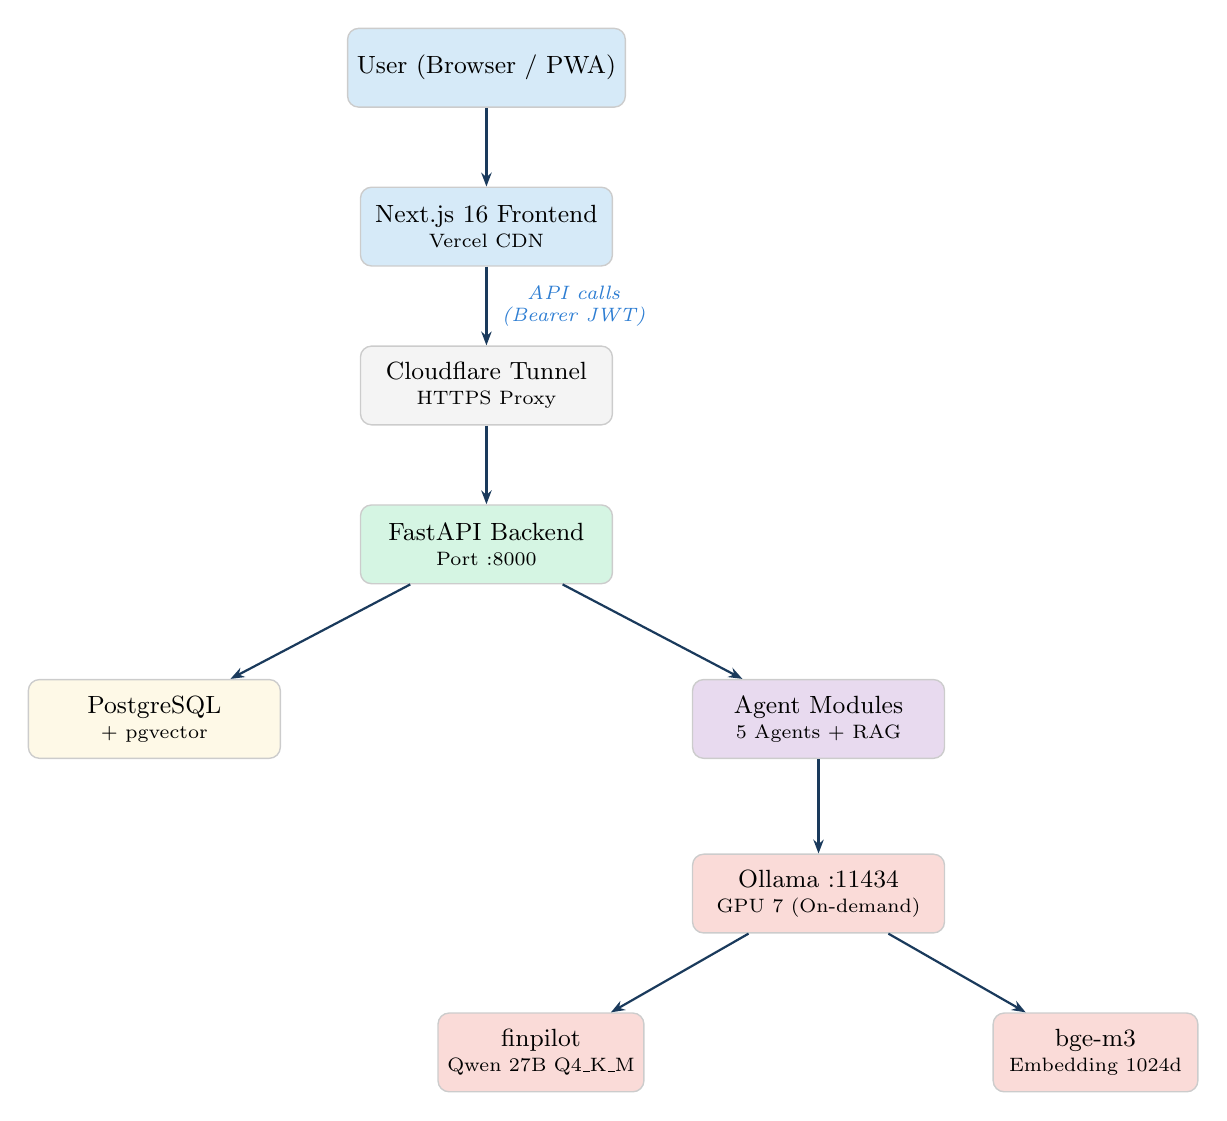
\begin{tikzpicture}[
  node distance=1.0cm and 1.8cm,
  every node/.style={
    font=\small,
    align=center,
    rounded corners=4pt,
    minimum height=1.0cm,
    minimum width=3.2cm,
    draw=midgray,
    line width=0.5pt
  },
  arr/.style={
    -{Stealth[length=5pt]},
    thick,
    color=primary
  },
  label/.style={
    font=\scriptsize\itshape,
    text=accent,
    fill=none,
    draw=none,
    minimum height=0pt,
    minimum width=0pt
  }
]

% Row 1: Client
\node[fill=nodeblue] (client) {User (Browser / PWA)};

% Row 2: Frontend
\node[fill=nodeblue, below=of client] (frontend)
  {Next.js 16 Frontend\\[-2pt]\scriptsize Vercel CDN};

% Row 3: Tunnel
\node[fill=lightgray, below=of frontend] (tunnel)
  {Cloudflare Tunnel\\[-2pt]\scriptsize HTTPS Proxy};

% Row 4: Backend
\node[fill=nodegreen, below=of tunnel] (backend)
  {FastAPI Backend\\[-2pt]\scriptsize Port :8000};

% Row 5 branches
\node[fill=nodeyellow, below left=1.2cm and 1.0cm of backend] (db)
  {PostgreSQL\\[-2pt]\scriptsize + pgvector};
\node[fill=nodepurple, below right=1.2cm and 1.0cm of backend] (agents)
  {Agent Modules\\[-2pt]\scriptsize 5 Agents + RAG};

% Row 6: Ollama
\node[fill=nodered, below=1.2cm of agents] (ollama)
  {Ollama :11434\\[-2pt]\scriptsize GPU 7 (On-demand)};

% Row 7 branches
\node[fill=nodered, below left=1.0cm and 0.6cm of ollama,
      minimum width=2.6cm] (finpilot)
  {finpilot\\[-2pt]\scriptsize Qwen 27B Q4\_K\_M};
\node[fill=nodered, below right=1.0cm and 0.6cm of ollama,
      minimum width=2.6cm] (bgem3)
  {bge-m3\\[-2pt]\scriptsize Embedding 1024d};

% Arrows
\draw[arr] (client)   -- (frontend);
\draw[arr] (frontend)  -- node[label, right, xshift=2pt]
           {API calls\\(Bearer JWT)} (tunnel);
\draw[arr] (tunnel)    -- (backend);
\draw[arr] (backend)   -- (db);
\draw[arr] (backend)   -- (agents);
\draw[arr] (agents)    -- (ollama);
\draw[arr] (ollama)    -- (finpilot);
\draw[arr] (ollama)    -- (bgem3);

\end{tikzpicture}
\caption{BizPlot system architecture and request flow.}
\label{fig:arch}
\end{figure}


% ══════════════════════════════════════════════════════════
\section{Frontend}
% ══════════════════════════════════════════════════════════

The client application is a Progressive Web App deployed on Vercel,
supporting home-screen installation on both iOS and Android.

\begin{table}[H]
\centering
\caption{Frontend technology stack.}
\label{tab:frontend}
\renewcommand{\arraystretch}{1.35}
\begin{tabularx}{\textwidth}{M{3.0cm} L}
\toprule
\textbf{Component}  & \textbf{Detail} \\
\midrule
Framework       & Next.js 16.2.6 (App Router), React 19, TypeScript \\
Styling         & Tailwind CSS v4 with PostCSS and custom design tokens
                  defined in \texttt{globals.css} \\
UI Libraries    & Radix UI (dialog, tabs, tooltip), Lucide React (icons),
                  Recharts (charts), Framer Motion (animation) \\
XAI Views       & Custom SVG/CSS causal-attribution graph
                  (\texttt{CausalFlowGraph}): a measured-edge DAG on desktop
                  and a 100\% stacked composition bar on mobile, plus
                  expandable per-strategy rationale panels \\
HTTP Client     & Axios with Bearer token interceptor
                  (\texttt{lib/api.ts}) \\
PWA Support     & \texttt{manifest.json} and \texttt{sw.js} service worker;
                  install banner shown once per login session on iOS and
                  Android (\texttt{sessionStorage} guard) \\
Deployment      & Vercel (Incheon edge, automatic HTTPS and CDN) \\
API Connection  & \texttt{NEXT\_PUBLIC\_API\_URL} pointing to
                  \texttt{https://api.bizplot.co.kr/api} with cross-origin
                  Bearer authentication \\
\bottomrule
\end{tabularx}
\end{table}


% ══════════════════════════════════════════════════════════
\section{Backend}
% ══════════════════════════════════════════════════════════

The backend is a Python service running on a GPU-enabled host,
exposed to the internet through a Cloudflare Tunnel.

\begin{table}[H]
\centering
\caption{Backend technology stack.}
\label{tab:backend}
\renewcommand{\arraystretch}{1.35}
\begin{tabularx}{\textwidth}{M{3.0cm} L}
\toprule
\textbf{Component}  & \textbf{Detail} \\
\midrule
Framework       & FastAPI with Uvicorn on port 8000, exposed through
                  Cloudflare Tunnel \\
Database        & PostgreSQL with the pgvector extension (1024-dimensional
                  embeddings), SQLAlchemy ORM, Alembic migrations \\
Authentication  & JWT Bearer tokens (\texttt{core/security.py}),
                  bcrypt password hashing \\
Configuration   & Pydantic Settings loading from
                  \texttt{backend/.env} \\
Background Jobs & FastAPI \texttt{BackgroundTasks} for diagnosis and
                  report generation via
                  \texttt{agent/report/review\_worker} \\
External Data   & Korea Open Data Portal (\texttt{data.go.kr}),
                  KOSIS (commercial district and statistics),
                  Kakao and Google APIs (geocoding and place search) \\
Exports         & PDF and CSV generation and download through
                  \texttt{routes/export.py} and
                  \texttt{report\_worker.py} \\
\bottomrule
\end{tabularx}
\end{table}


% ══════════════════════════════════════════════════════════
\section{AI Pipeline}
% ══════════════════════════════════════════════════════════

\subsection{Base Model and Fine-Tuning}

The core language model is Qwen 3.6-27B, fine-tuned using QLoRA
on a single NVIDIA A6000 GPU (48\,GB VRAM).
Table~\ref{tab:finetune} summarizes the training configuration.

\begin{table}[H]
\centering
\caption{QLoRA fine-tuning configuration.}
\label{tab:finetune}
\renewcommand{\arraystretch}{1.35}
\begin{tabularx}{\textwidth}{M{3.6cm} L}
\toprule
\textbf{Parameter}       & \textbf{Value} \\
\midrule
Base Model               & Qwen/Qwen3.6-27B (27 billion parameters) \\
Quantization             & BitsAndBytes NF4 4-bit with double quantization,
                           compute dtype bfloat16 \\
LoRA Rank / Alpha        & $r = 16$, $\alpha = 32$, dropout $= 0.05$ \\
Target Modules           & All attention and MLP projections
                           (q, k, v, o, gate, up, down) \\
Trainer                  & TRL SFTTrainer \\
Sequence Length           & 2048 tokens \\
Effective Batch Size     & 8 (micro-batch 1 $\times$ gradient accumulation 8) \\
Learning Rate            & $2 \times 10^{-4}$ with cosine schedule \\
Training Duration        & 3 epochs, capped at 300 steps \\
Optimizer                & Paged AdamW 8-bit \\
Hardware                 & NVIDIA A6000 48\,GB (GPU slot 2) \\
\bottomrule
\end{tabularx}
\end{table}


\subsection{Training Data}

Synthetic instruction data is generated by
\texttt{create\_training\_data.py}.
The corpus contains over 500 examples spanning multiple business
categories, formatted as multi-turn chat sequences
(system, user, assistant) with structured JSON outputs for
diagnosis and strategy tasks.
Output files reside at
\texttt{data/training/\{train,val\}.jsonl}.


\subsection{Post-Training Pipeline}

Table~\ref{tab:pipeline} shows the conversion steps from the
fine-tuned adapter to the final quantized model served in production.

\begin{table}[H]
\centering
\caption{Model conversion pipeline.}
\label{tab:pipeline}
\renewcommand{\arraystretch}{1.35}
\begin{tabularx}{\textwidth}{M{0.6cm} M{3.4cm} L}
\toprule
\textbf{\#} & \textbf{Stage} & \textbf{Output} \\
\midrule
1 & QLoRA SFT              & LoRA adapter weights
                             (\texttt{final\_adapter}) \\
2 & Merge and Unload       & Full bfloat16 model
                             (\texttt{finpilot-qwen3.6-27b-merged}) \\
3 & llama.cpp Conversion   & \texttt{finpilot-bf16.gguf} \\
4 & Q4\_K\_M Quantization  & \texttt{finpilot-q4km.gguf}
                             (served by Ollama) \\
\bottomrule
\end{tabularx}
\end{table}

\subsection{Chinese Character Post-Processing}

Qwen occasionally inserts Chinese characters and full-width
punctuation into Korean-language output.
A dedicated filter, \texttt{llm\_client.strip\_chinese()},
removes these artifacts from every \texttt{call\_llm} response
before JSON parsing.


\subsection{Explainable AI (XAI)}
\label{sec:xai}

A central design principle separates \emph{deterministic computation}
from \emph{model-generated narration}: every numeric quantity shown to
the user is derived by deterministic code, while the language model
only produces grounded natural-language explanations on top of those
numbers. This keeps the figures auditable and reproducible while still
delivering rich, readable reasoning.

\textbf{Causal attribution graph.}
The \texttt{causal\_analysis} agent expresses revenue change as a
three-tier graph: data evidence $\rightarrow$ causal factor
$\rightarrow$ revenue/cash outcome. The revenue delta is first
decomposed by a sales bridge (volume/traffic effect versus unit-price
effect); the volume effect is then distributed across measured drivers
(in-radius competition, time-of-day demand, weather, and review
sentiment) in proportion to their quantified scores. Each factor's
contribution equals the sum of its child evidence weights, so
contributions are additive and always total 100\%. The model narrates
only the one-line factor and summary text; it never invents the
percentages. The graph is stored inside the existing
\texttt{Diagnosis.causes} JSONB column (with nested \texttt{evidence}
and \texttt{group} fields), requiring no schema migration.

\textbf{Strategy rationale.}
After the strategies are finalized, \texttt{strategy\_planner} issues a
dedicated grounded-generation call (\texttt{\_attach\_rationales}): the
model receives the store's financial state, the diagnosed causes with
their contribution percentages and supporting evidence, and each
recommended action with its expected impact, then writes five to six
explanation lines per strategy. Each line covers a distinct angle---the
diagnosed cause it targets and that cause's contribution, the specific
past-data evidence, the operating mechanism, the expected impact
converted to a won figure against recent revenue, why the figure is
realistic, and the metric to verify afterwards. The prompt forbids
repeated phrasing across strategies and restricts the model to the
supplied numbers. The parsed output is stored in each action's
\texttt{rationale} field (JSONB, no migration). If the model output is
missing or too thin, the frontend falls back to a deterministic
explanation builder (\texttt{lib/strategyXai.ts}) so an explanation is
always present. Because the diagnosis worker re-runs strategy planning,
the rationale is regenerated automatically on every re-diagnosis.


% ══════════════════════════════════════════════════════════
\section{Agent Modules}
% ══════════════════════════════════════════════════════════

The backend exposes five specialized agents, each responsible
for a distinct analytical task.

\begin{table}[H]
\centering
\caption{Agent module descriptions.}
\label{tab:agents}
\renewcommand{\arraystretch}{1.35}
\begin{tabularx}{\textwidth}{M{3.4cm} L}
\toprule
\textbf{Agent}           & \textbf{Responsibility} \\
\midrule
\texttt{finance\_state}     & Compute financial health indicators from
                              uploaded business data \\
\texttt{causal\_analysis}   & Decompose revenue decline into additive
                              contribution factors via a deterministic
                              evidence $\rightarrow$ factor $\rightarrow$
                              outcome attribution graph (the model narrates
                              text only; see Section~\ref{sec:xai}) \\
\texttt{strategy\_planner}  & Generate operational, marketing, and
                              financial strategies, each with a
                              model-generated, data-grounded rationale (XAI)
                              and a deterministic fallback \\
\texttt{review\_analysis}   & Perform sentiment analysis and keyword
                              extraction on customer reviews \\
\texttt{rag\_agent}         & Retrieve relevant government subsidy
                              and financial product information \\
\bottomrule
\end{tabularx}
\end{table}


% ══════════════════════════════════════════════════════════
\section{RAG System}
% ══════════════════════════════════════════════════════════

Retrieval-Augmented Generation is used to ground strategy
recommendations in real policy documents and financial products.

\subsection{Embedding and Storage}

\begin{table}[H]
\centering
\caption{RAG embedding and storage configuration.}
\label{tab:rag}
\renewcommand{\arraystretch}{1.35}
\begin{tabularx}{\textwidth}{M{3.0cm} L}
\toprule
\textbf{Component}   & \textbf{Detail} \\
\midrule
Embedding Model      & bge-m3 (1024 dimensions, multilingual with
                       Korean support), served via Ollama
                       \texttt{/api/embeddings} \\
Transport            & httpx (no PyTorch dependency, resilient to
                       CUDA conflicts) \\
Vector Store         & PostgreSQL pgvector table
                       \texttt{rag\_documents} with column type
                       \texttt{vector(1024)} \\
Similarity Metric    & Cosine distance (\texttt{<=>} operator),
                       top-K retrieval \\
Fallback             & Korean keyword search with title weighting
                       ($\times 3$) and body term frequency
                       (BM25-style) when embedding service is
                       unavailable \\
\bottomrule
\end{tabularx}
\end{table}

\subsection{Corpus Ingestion}

Documents are prepared in two stages.
First, \texttt{build\_rag\_corpus.py} assembles the raw corpus
from small business support programs, consultation guides, and
JB Financial Group product sheets (tagged with
\texttt{source = jb}).
Then, \texttt{ingest\_rag.py} generates embeddings and inserts
records into the database.
During diagnosis, the user's business category is mapped to
Korean keywords to retrieve the most relevant policy documents
for strategy grounding.


% ══════════════════════════════════════════════════════════
\section{Ollama Serving Layer}
% ══════════════════════════════════════════════════════════

Ollama provides an OpenAI-compatible API on port 11434, backed by
the llama.cpp runtime.
This eliminates the need for a PyTorch runtime in the serving path.

\begin{table}[H]
\centering
\caption{Ollama serving configuration.}
\label{tab:ollama}
\renewcommand{\arraystretch}{1.35}
\begin{tabularx}{\textwidth}{M{3.0cm} L}
\toprule
\textbf{Parameter}     & \textbf{Value} \\
\midrule
Inference Model        & \texttt{finpilot} (Qwen 27B, Q4\_K\_M GGUF) \\
Embedding Model        & bge-m3 (1024 dimensions) \\
Generation Config      & temperature 0.2, top-p 0.9,
                         context window 8192 tokens \\
Concurrency            & Up to 4 parallel batched requests \\
VRAM Management        & On-demand loading to GPU 7, automatic unload
                         after 5 minutes of idle time \\
Backend Call Path       & \texttt{call\_llm} uses the OpenAI SDK
                         targeting
                         \texttt{localhost:11434/v1/chat/completions} \\
Embedding Call Path    & \texttt{get\_embedding} calls
                         \texttt{localhost:11434/api/embeddings} \\
Model Definition       & Custom \texttt{Modelfile} specifying the GGUF
                         path, generation parameters, stop tokens, and
                         system prompt \\
\bottomrule
\end{tabularx}
\end{table}


% ══════════════════════════════════════════════════════════
\section{Deployment Topology}
% ══════════════════════════════════════════════════════════

Table~\ref{tab:deploy} provides a summary of where each major
component runs and how they interconnect.

\begin{table}[H]
\centering
\caption{Deployment locations and connectivity.}
\label{tab:deploy}
\renewcommand{\arraystretch}{1.35}
\begin{tabularx}{\textwidth}{M{2.8cm} M{2.6cm} L}
\toprule
\textbf{Component} & \textbf{Location} & \textbf{Connectivity} \\
\midrule
Next.js Frontend   & Vercel CDN (Incheon edge)
                   & Calls \texttt{api.bizplot.co.kr} over HTTPS \\
Cloudflare Tunnel  & Cloudflare Network
                   & Routes \texttt{api.bizplot.co.kr} to
                     backend port 8000 \\
FastAPI Backend    & GPU Backend Host
                   & Connects to local PostgreSQL and Ollama on port 11434 \\
PostgreSQL         & GPU Backend Host
                   & pgvector extension for 1024-d vectors \\
Ollama             & GPU Backend Host (GPU 7)
                   & Serves \texttt{finpilot} and \texttt{bge-m3}
                     on port 11434 \\
\bottomrule
\end{tabularx}
\end{table}


\end{document}
